\section{Prototypical Networks (Protonets)~\cite{prototypical}}

\textbf{Goals:} In this assignment, you will experiment with a meta-learning algorithms - prototypical networks (protonets)~\cite{prototypical} for few-shot image classification on the Omniglot dataset \cite{Lake1332}. You will:
\begin{enumerate}
    \item Implement the protonets algorithms (given starter code).
    \item Interpret key metrics of the algorithm.
    \item Investigate the effect of task composition during protonet training on evaluation.
    \item Investigate the performance of the algorithm on meta-test tasks that have more support data than training tasks do.
\end{enumerate}

\textbf{Expectations}
\begin{itemize}
    \item We expect you to develop your solutions locally (i.e. make sure your model can run for a few training iterations), but to use GPU-accelerated training (e.g. Google Colab, Azure) for your results.
\end{itemize}

\textbf{Notation}
\begin{itemize}
    \item $x$: Omniglot image
    \item $y$: class label
    \item $N$ (way): number of classes in a task
    \item $K$ (shot): number of support examples per class
    \item $Q$: number of query examples per class
    \item $c_n$: prototype of class $n$
    \item $f_\theta$: neural network parameterized by $\theta$
    \item $\task_i$: task $i$
    \item $\supportdata_i$: support data in task $i$
    \item $\querydata_i$: query data in task $i$
    \item $B$: number of tasks in a batch
    \item $\mathcal{J}(\theta)$: objective function parameterized by $\theta$
\end{itemize}

For this assignment, please submit the following files to gradescope to recieve points for coding questions:
\begin{itemize}
    \item |submission.pdf|
    \item |src/submission/__init__.py|
    \item |src/submission/maml.py|
    \item |src/submission/maml_results_1_5_1_0.4_False.npy|
    \item |src/submission/maml_results_1_5_1_0.04_False.npy|
    \item |src/submission/maml_results_1_5_1_0.4_True.npy|
    \item |src/submission/maml_results_1_5_5_0.04_False.npy|
    \item |src/submission/protonet.py|
    \item |src/submission/protonet_results_1_5.npy|
    \item |src/submission/protonet_results_5_5.npy|
\end{itemize}

\newpage

\subsubsection*{Protonets Algorithm Overview}
\begin{figure}[H]
\centering
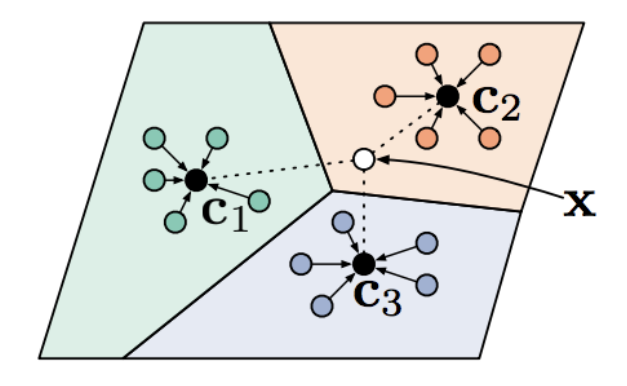
\includegraphics[width=0.5\linewidth]{./figures/protonets}
\vspace{-3mm}
\caption{Prototypical networks in a nutshell. In a 3-way 5-shot classification task, the class prototypes $c_1, c_2, c_3$ are computed from each class's support features (colored circles). The prototypes define decision boundaries based on Euclidean distance. A query example $x$ is determined to be class 2 since its features (white circle) lie within that class's decision region.}
\label{fig:protonet}
\end{figure}

As discussed in lecture, the basic idea of protonets is to learn a mapping $f_\theta(\cdot)$ from images to features such that images of the same class are close to each other in feature space. Central to this is the notion of a \emph{prototype}
\begin{equation}
    c_n = \frac{1}{K} \sum_{(x,y) \in \supportdata_i : y = n} f_\theta(x),
\end{equation}
i.e. for task $i$, the prototype of the $n$-th class $c_n$ is defined as the mean of the $K$ feature vectors of that class's support images.
To classify some image $x$, we compute a measure of distance $d$ between $f_\theta(x)$ and each of the prototypes. We will use the squared Euclidean distance:
\begin{equation}
    d(f_\theta(x), c_n) = \| f_\theta(x) - c_n \|_2^2.
\end{equation}
We interpret the negative squared distances as logits, or unnormalized log-probabilities, of $x$ belonging to each class. To obtain the proper probabilities, we apply the softmax operation:
\begin{equation}
    p_\theta(y=n \mid x) = \frac{\exp(-d(f_\theta(x), c_n))}{\sum_{n'=1}^N \exp(-d(f_\theta(x), c_{n'}))}.
\end{equation}
Because the softmax operation preserves ordering, the class whose prototype is closest to $f_\theta(x)$ is naturally interpreted as the most likely class for $x$. To train the model to generalize, we compute prototypes using support data, but minimize the negative log likelihood of the query data
\begin{equation}
    \mathcal{J}(\theta) = \E_{\task_i \sim p(\task), (\supportdata_i, \querydata_i) \sim \task_i} \left[ \frac{1}{NQ} \sum_{(\query{x},\query{y}) \in \querydata_i} - \log p_\theta(y = \query{y} \mid \query{x}) \right].
    \label{eq:protonet_objective}
\end{equation}

Notice that this is equivalent to using a cross-entropy loss.

We optimize $\theta$ using Adam~\cite{kingma2014adam}, an off-the-shelf gradient-based optimization algorithm.
As is standard for stochastic gradient methods, we approximate the objective~\eqref{eq:protonet_objective} with Monte Carlo estimation on minibatches of tasks. For one minibatch with $B$ tasks, we have

\begin{equation}
    \mathcal{J}(\theta) \approx \frac{1}{B} \sum_{i=1}^B 
     \left[ \frac{1}{NQ} \sum_{(\query{x},\query{y}) \in \querydata_i} - \log p_\theta(y = \query{y} \mid \query{x}) \right].
    \label{eq:protonet_objective_minibatch}
\end{equation}

\begin{enumerate}[label={1.\alph*}]
	\item \points{1a} {\bf No Shuffle Required}

We have provided you with \texttt{omniglot.py}, which contains code for task construction and data loading.

Recall that for training black-box meta-learners in the previous homework we needed to shuffle the query examples in each task. This is not necessary for training protonets. Explain why.
    \item \points{1b} {\bf Implement Step}

In the \texttt{protonet.py} file, complete the implementation of the \texttt{ProtoNet.\_step} method, which computes \eqref{eq:protonet_objective_minibatch} along with accuracy metrics. Pay attention to the inline comments and docstrings.
    
Assess your implementation on 5-way 5-shot Omniglot. To do so, run 
\begin{equation*} 
    \texttt{python protonet.py --num\_support 5} 
\end{equation*}

Use 15 query examples per class per task. Depending on how much memory your GPU has, you may want to adjust the batch size. Do not adjust the learning rate from its default of $0.001$.

To specify a non-default value for an argument, use the following syntax:
\begin{equation*}
    \texttt{python protonet.py --argument1 value1 --argument2 value2}
\end{equation*}

    As the model trains, model checkpoints and TensorBoard logs are periodically saved to a \texttt{log\_dir}. The default \texttt{log\_dir} is formatted from the arguments, but this can be overriden. You can visualize logged metrics by running
\begin{equation*}
    \texttt{tensorboard --logdir logs/}
\end{equation*}
and navigating to the displayed URL in a browser. If you are running on a remote computer with server capabilities, use the \texttt{--bind\_all} option to expose the web app to the network. Alternatively, consult the Azure guide for an example of how to tunnel/port-forward via SSH.

To resume training a model starting from a checkpoint at \texttt{\{some\_dir\}/state\{some\_step\}.pt}, run
\begin{equation*}
    \texttt{python protonet.py --log\_dir some\_dir --checkpoint\_step some\_step}
\end{equation*}

Your plot of the validation query accuracy over the course of training should look like the figure below.
\begin{center}
    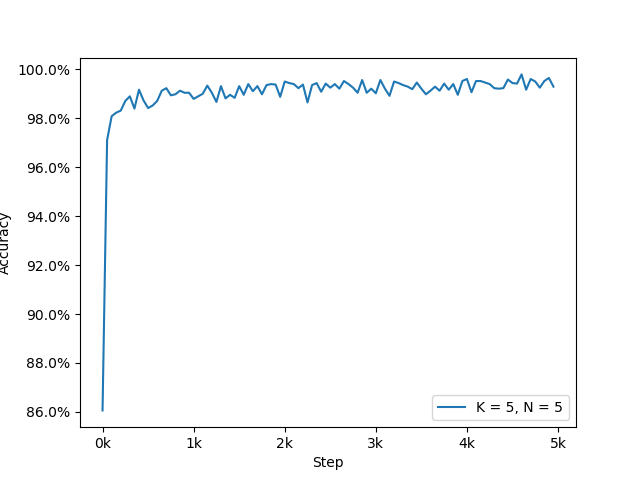
\includegraphics[width=0.75\linewidth]{./figures/protonets_q2}
\end{center}

\textbf{Hint}: you should obtain a query accuracy on the validation split of at least $99\%$.
    \item \points{1c} {\bf Evaluating Accuracy Metrics}

4 accuracy metrics are logged. For the above run, examine these in detail to reason about what the algorithm is doing.

\begin{enumerate}[label=(\roman*)]
    \item Is the model placing support examples of the same class close together in feature space or not? Support your answer by referring to specific accuracy metrics.
    
    \item Is the model generalizing to new tasks? If not, is it overfitting or underfitting? Support your answer by referring to specific accuracy metrics.
\end{enumerate}
    \item \points{1d} {\bf 5-way 1-shot Comparison}
We will now compare different settings at training time. Train on 5-way 1-shot tasks with 15 query examples per task. 
\begin{enumerate}[label=(\roman*)]
    \item Compare your two runs (5-way 1-shot training and 5-way 5-shot training) by assessing test performance on 5-way 1-shot tasks. To assess a trained model on test tasks, run
    \begin{equation*}
        \texttt{python protonet.py --test}
    \end{equation*}

    appropriately specifying \texttt{log\_dir} and \texttt{checkpoint\_step}. Submit a table of your results with 95\% confidence intervals.
        
    \item How did you choose which checkpoint to use for testing for each model? 
        
    \item Is there a significant difference in the test performance on 5-way 1-shot tasks? Explain this by referring to the protonets algorithm.
\end{enumerate}
\end{enumerate}